\section{\index{Backend Architecture}Backend Architecture Specifications}

\begin{itemize}
    \item There are $n$ buses: $0, 1, 2, \ldots n-1$
    \item There are $m$ stops: $0, 1, 2, \ldots m-1$  ($0$: first stop, $m-1$: last stop)
    \item We have to synchronize the \textit{\gls{24-hour clock}} at each stop
    \item In this system, all bus shifts end at the starting stop, i.e. the bus shift ends when the bus is back at the $0$\textsuperscript{th} stop. The sequence followed in a shift is \\
          {\bfseries $0$ $\to$ $1$ $\to$ $2$ $\to$ $3$ $\to$ \ldots $\to$ $m-2$ $\to$ $m-1$ $\to$ $m-2$ $\to$ \ldots$\to$ $3$ $\to$ $2$ $\to$ $1$ $\to$ $0$}\\
\end{itemize}

\begin{figure}[H]
        \centering
        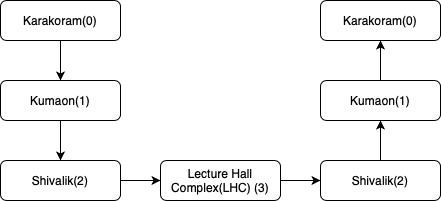
\includegraphics[width=0.7\textwidth]
        {./Files/Images/Flowchart.png}
        \caption{\textbf{Example route for m = 4}} % Add a caption
    \end{figure}

\begin{itemize}
    \item All these stops will be connected to the institute’s WiFi service, which will be used to transmit relevant information to all the stops 
    \item⁠ We use WiFi even when the ESP32 has the option of BLE because:
\begin{itemize}
    \item BLEs indoor range is around 100 m, but outdoors the signals are attenuated and therefore the range reduces
    \item We need to cover a route of approximately 2 km using 4 bus units. Therefore using BLE is not feasible unless we can have bus stops every 50-100 metres, which seems impractical.
\end{itemize}
\end{itemize}
\subsection{Data Storage and Timing Estimates}
\subsubsection{Over the Network}

\begin{enumerate}

\item Maintain the \textbf{Arrival}\textsubscript{mxn} matrix : Element $(i, j)$ stores the arrival time of $j$\textsuperscript{th} bus at the $i$\textsuperscript{th} stop
\item Maintain the \textbf{Departure}\textsubscript{mxn} matrix : Element $(i, j)$ stores the departure time of $j$\textsuperscript{th} bus at the $i$\textsuperscript{th} stop
\item Maintain the \textbf{PassengerWaitingAtStop}\textsubscript{1xm} matrix : Element $(0, j)$ is $x$ where
 \[ x = \begin{cases} \mbox{1} & \mbox{if any passenger is waiting at the j\textsuperscript{th} stop}  \\ \mbox{0} & \mbox{otherwise} \end{cases} \]
\item Maintain the \textbf{Direction}\textsubscript{1xn} matrix : Element (0, j) is x where
 \[ x = \begin{cases} \mbox{0} & \mbox{if $j$\textsuperscript{th} bus is moving towards $0$\textsuperscript{th} stop}  \\ \mbox{1} & \mbox{if $j$\textsuperscript{th} bus is moving towards $m-1$\textsuperscript{th} stop} \end{cases} \]


\end{enumerate}
\subsubsection{Locally}

\begin{itemize}

\item Maintain the \textbf{Scheduled}\textsubscript{mxn} matrix: Element (i, j) stores the scheduled time of the j\textsuperscript{th} bus at the i\textsuperscript{th} stop.
\item Maintain the \textbf{Estimated}\textsubscript{mxn} matrix: Element (i, j) stores the estimated time of the j\textsuperscript{th} bus at the i\textsuperscript{th} stop.
\item These matrices can be stored for estimation of arrival times, the passenger waiting functionality.
\item When j\textsuperscript{th} bus arrives at the i\textsuperscript{th} stop: (i, j)\textsuperscript{th} element of the \textbf{Arrival} matrix is updated. Bus stop `i' acts as the server, and all other bus stops act as clients.
\item When j\textsuperscript{th} bus departs the i\textsuperscript{th} stop: (i, j)\textsuperscript{th} element is updated. All arrival times of j\textsuperscript{th} column are updated to new estimate times based on \textit{average} time between stops and departure time from i\textsuperscript{th} stop.
\item For sensing whether the bus has stopped or not, we are using \textit{Accelerometer} reading.
\item \textbf{Bus stop nodes that can access this matrix} (i.e. nodes that are connected to the network):\\
\null \qquad Arrival time of next bus at i\textsuperscript{th} stop= min\{i\textsuperscript{th} row\}\\
\null \qquad Suppose that j the next bus arriving at i\textsuperscript{th} stop = j.\\
\null \qquad Direction of next bus = j\textsuperscript{th} element of \textbf{Direction} matrix.\\
\null \qquad Both Arrival time and Direction of buses needs to be communicated to the commuters.

\item \textbf{Bus stop nodes that cannot access this matrix} (i.e. nodes that unexpectedly get disconnected):\\
\null \qquad Arrival times of each bus estimated using scheduled time and last known whereabouts of buses:\\
\null \qquad \qquad Estimated time = Scheduled time + (last known deviation from scheduled\\
\null \qquad \qquad time)\\
\null \qquad If estimated time shows a large deviation from scheduled time, we will use scheduled time instead of estimated time.\\
\null \qquad Direction matrix can be updated based on these estimates: Direction of j\textsuperscript{th} bus switches when arrival time of stop m-1 is crossed.\\
\null \qquad Similar to the previous case, both Arrival time and Direction of buses needs to be communicated to the commuters.

\item \textbf{When the bus reaches stop 0 after a round trip}:\\
\null \qquad The \textbf{Arrival} and \textbf{Departure} matrices are updated to actual/estimated arrival and departure values, and this can be used to keep log of actual arrival and departure times in the system.\\
\null \qquad Moving average of previous runs can be used to refine predictions.\\
\null \qquad After uploading these times, we reset \textbf{Arrival} and \textbf{Departure} matrices to scheduled times.

\item \textbf{For more frequent time updates:}\\
\null \qquad We can specify some locations (using \textit{GPS}) where Wi-Fi is available on the route and send quick location updates to the network.\\
\null \qquad These locations can be used as \textit{pseudo-stops}, where the Bus Unit directly informs all Bus Stop nodes its location which can be further used to refine time predictions.
\end{itemize}
\subsection{Passenger waiting problem}

\begin{enumerate}

    \item We can use an \gls{ultrasonic sensor} at each stop to detect any passenger standing within 5 feet of the bus stop. If the sensor detects an obstacle within 5 feet for more than 30 seconds, then the (0, j)\textsuperscript{th} entry of \textbf{PassengerWaitingAtStop}\textsubscript{1xm} matrix is updated
    \item The bus unit stores a variable \textbf{PassengerWaiting} where\\
          \textbf{PassengerWaiting} = OR(all elements of \textbf{PassengerWaitingAtStop})
    \item This variable can be updated at every stop/pseudo stop

\end{enumerate}
\subsection{Protocol and Components}
The following are the possible network architectures we will be using:
\subsubsection{ESP NOW}
ESP-NOW is a wireless communication protocol based on the data-link layer, which reduces the five layers of the OSI model to only one. This way, the data need not be transmitted through the network layer, the transport layer, the session layer, the presentation layer, and the application layer. Also, there is no need for packet headers or unpackers on each layer, which leads to a quick response reducing the delay caused by packet loss in congested networks. 
\begin{figure}[H]
    \centering
    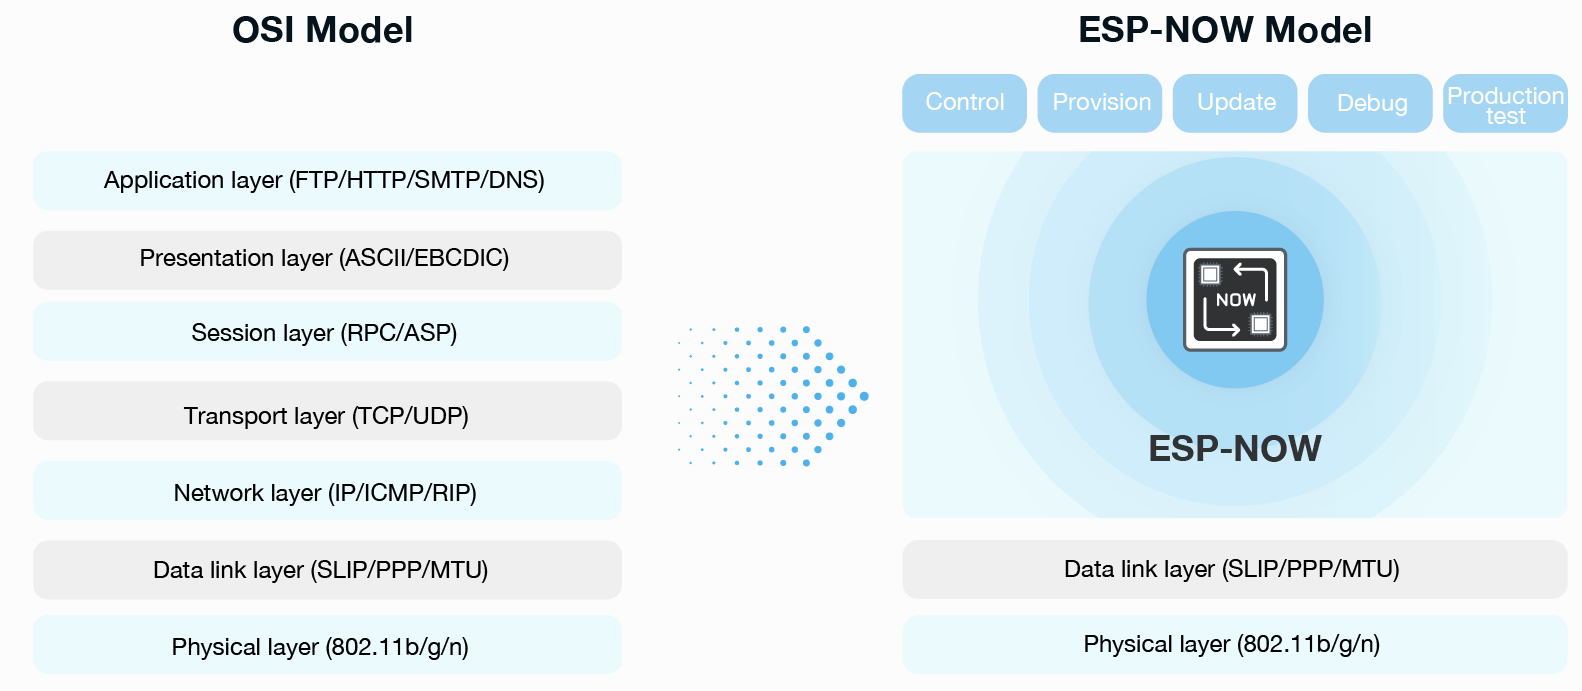
\includegraphics[width=0.75\linewidth]{Files/Images/model-en.png}
    \caption{Comparision of the OSI standard layers and the ESP NOW protocol layers}
    \label{fig:enter-label}
\end{figure}
Here are the key features of the ESP NOW Protocol:
\begin{itemize}
    \item It has a fast and user-friendly pairing method that is suitable for connecting “one-to-many” and “many-to-many” devices, while also controlling them
    \item Occupies fewer CPU and flash resources
    \item Can be used as an independent protocol that helps with device provisioning, debugging, and firmware upgrades
    \item  ECDH and AES algorithms make data transmission more secure
    \item The window synchronization mechanism greatly reduces power consumption
\end{itemize}
The devices communicates directly via the use of the data link and pairing do not require the Wi-Fi connection. Pairing can be done by initiating and multiple pairing can be done like one initiator can pair with multiple responder. Using the RSSI, during the paring the device distance can be found and that distance can be authorised and the device at that distance can be paired. The protocol supports long distance communication which will be helpful in using it outdoors. The portocol is compatible with many sensors implying its wide usability to interact among the units or the user and the unit. ESP NOW can also take data logs from multiple responders for analysis. This will facilitate the user to gather the data from the units without needing to go to the unit, again, the units can communicate the same among themselves to correctly estimate the time or find any abnormality in real time. 


\subsubsection{ESP-WIFI-MESH}
ESP-WIFI-MESH is a networking protocol that operates on top of the Wi-Fi protocol. It facilitates the interconnection of numerous devices, referred to as nodes, across a wide physical area, including both indoor and outdoor spaces, within a single WLAN (Wireless Local-Area Network).It is self-organizing and self-healing meaning the network can be built and maintained autonomously.

\begin{figure}[H]
     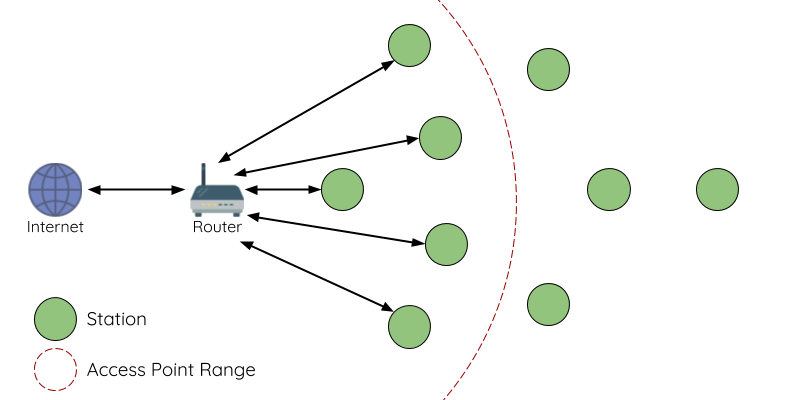
\includegraphics[width=0.5\linewidth]{Files/Images/traditional-network.png}
     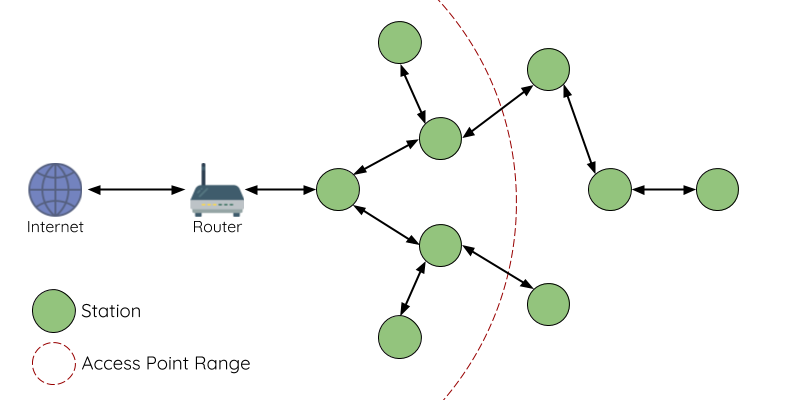
\includegraphics[width=0.55\linewidth]{Files/Images/esp-wifi-mesh.png}
     \caption{Traditional Wi-Fi Network vs ESP-WIFI-MESH Network}
     \label{fig:enter-label}

\end{figure}

Here are the key features of the ESP-WIFI-MESH:
\begin{itemize}
    \item ESP-WIFI-MESH networks do not rely on a central node like traditional infrastructure Wi-Fi networks. Instead, nodes connect with neighboring nodes, allowing for greater coverage area.
    \item Nodes within this network relay each other's transmissions, enabling interconnectivity without the need to be within range of a central node.
    \item Unlike traditional Wi-Fi networks, ESP-WIFI-MESH is not as susceptible to overloading since the number of nodes permitted on the network is not limited by a single central node's capacity.
\end{itemize}